\chapter{数学命题及解题教学心理}

\section{命题教学模式拓展}

命题学习——数学中的公理、定理、公式、法则、数学对象的性质等的学习

\subsection{数学命题学习的认知模式}

\[
\text{命题获得}\xrightarrow{}\text{命题证明}\xrightarrow{}\text{命题应用}
\]


\begin{enumerate}
    \item \textbf{命题获得}:
    \begin{itemize}
        \item 同化
        \item 形成
    \end{itemize}

    \item \textbf{命题证明}:
    \begin{itemize}
        \item 利用已获的命题,推证当前命题。
        \item 可用激活扩散模型解释。
    \end{itemize}

    \item \textbf{命题应用}:
    \begin{itemize}
        \item 解析性命题(公式法则)。
        \item 推理性命题(不含公式法则)。
    \end{itemize}
\end{enumerate}

\begin{figure}[H]
    \centering
    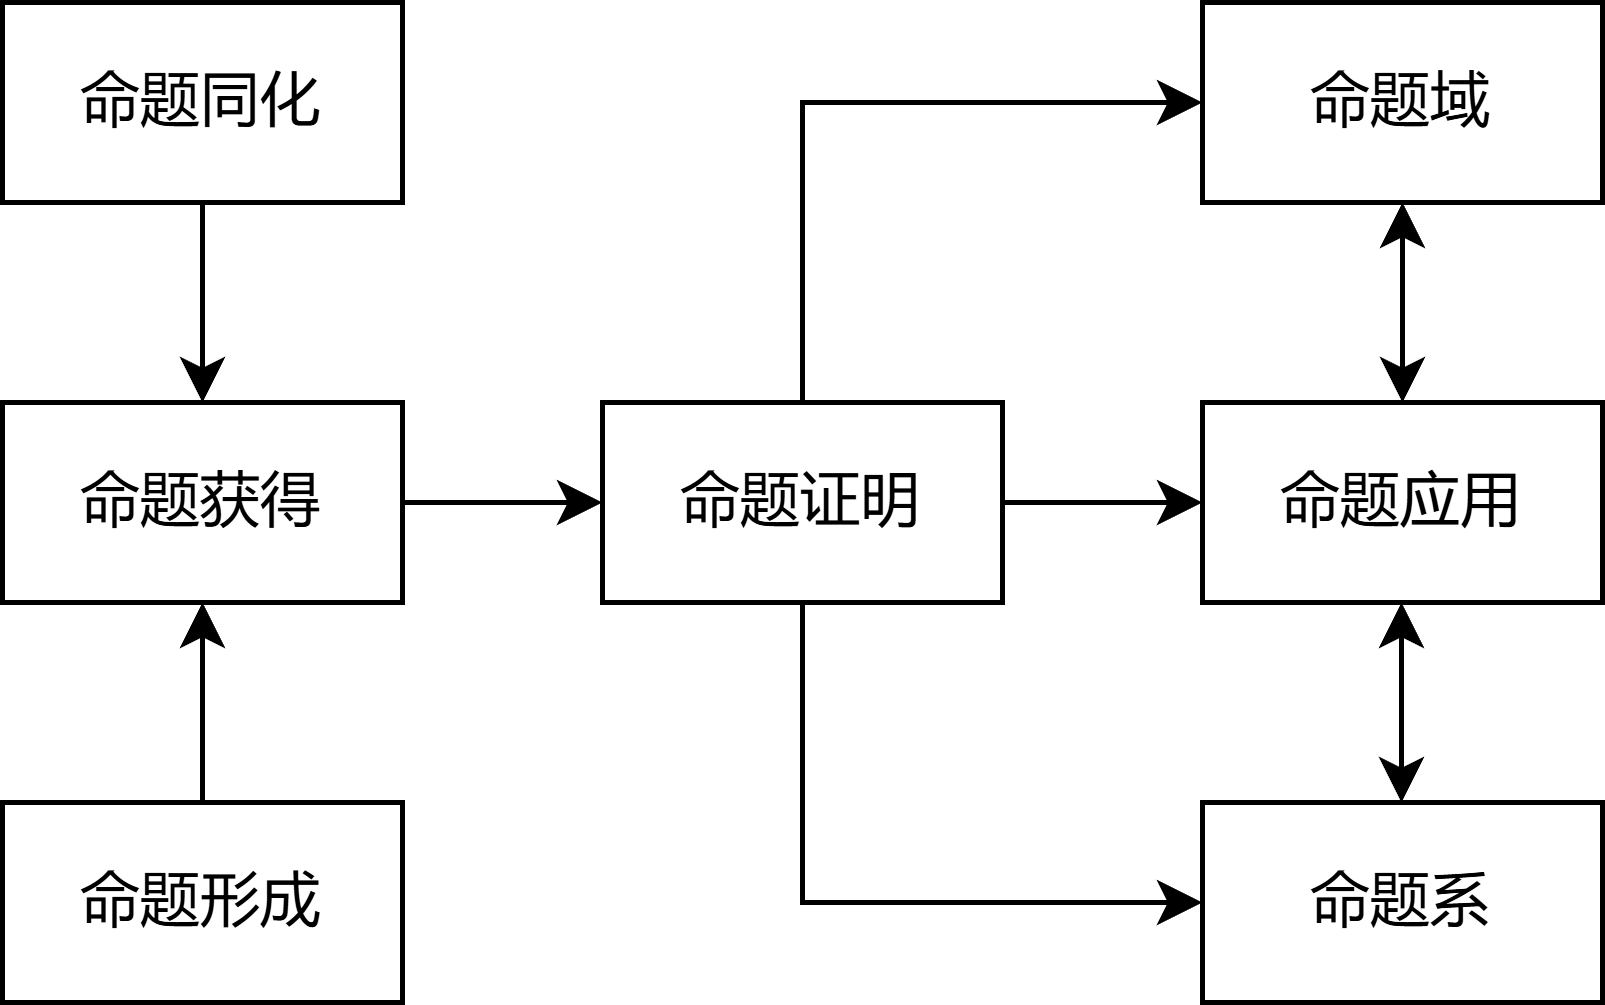
\includegraphics[width=0.45\linewidth]{image/数学命题学习过程.png}
\end{figure}



\subsection{数学命题学习的发生型模式}

通过揭示命题的产生过程去学习命题

\begin{figure}[H]
    \centering
    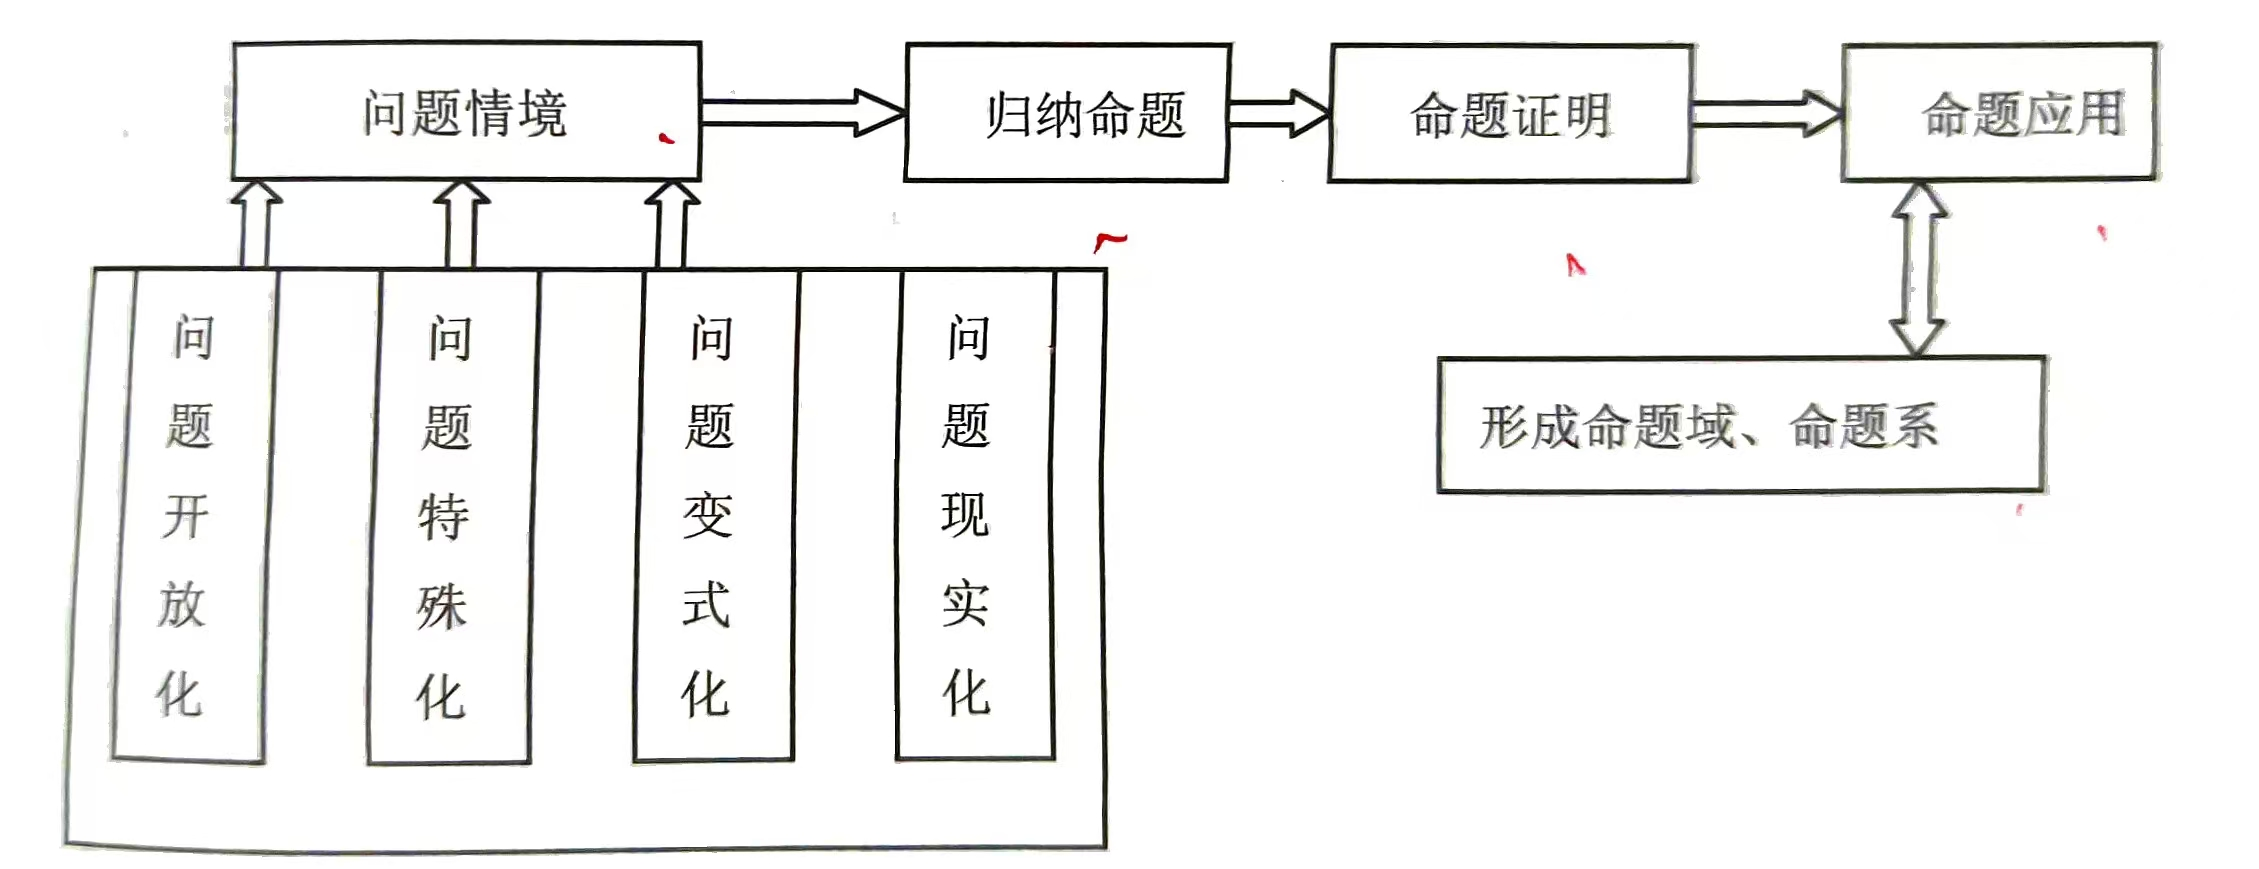
\includegraphics[width=0.5\linewidth]{image/fashengxingmoshi.jpg}
\end{figure}

\subsection{数学命题学习的结果型模式}

由教师直接展示命题去学习命题

\[
\text{展示命题}\xrightarrow{}\text{命题证明}\xrightarrow{}\text{命题应用}\longleftrightarrow\text{形成命题系(域)}
\]

\subsection{数学命题学习的问题解决模式}

通过解决问题引入命题

\begin{figure}[H]
    \centering
    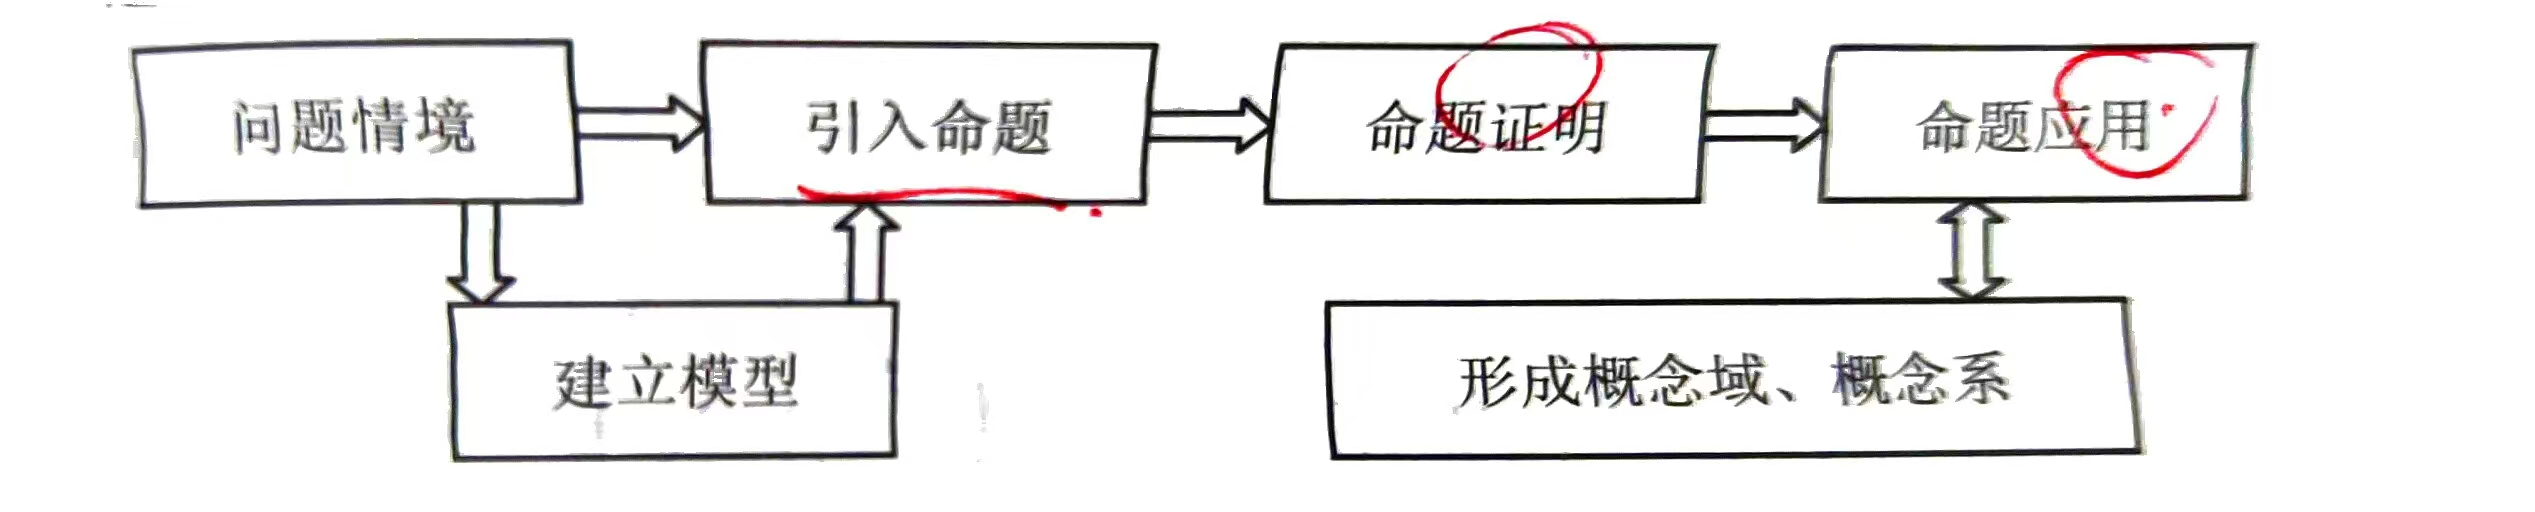
\includegraphics[width=0.5\linewidth]{image/wentijiejuemoshi.jpg}
\end{figure}


\subsection{数学命题教学策略}

\begin{enumerate}
    \item \textbf{注重过程}:
    \begin{itemize}
        \item 注重命题产生过程。
        \item 注重命题证明特征。
    \end{itemize}

    \item \textbf{注重变式}:
    \begin{itemize}
        \item \textbf{概念性变式}:用不同直观材料或事例说明事物本质属性,或变换其非本质属性以突出事物的本质特征。
        \item \textbf{过程性变式}:概念形成方面,要确保学生知到概念产生的缘由、体验知识形成过程;问题解决方面,注重对问题划归过程的解析。
    \end{itemize}

    \item \textbf{形成命题体系}:
    \begin{itemize}
        \item 命题的陈述性知识网络。
        \item 命题的程序性知识网络。
    \end{itemize}

    \item \textbf{加强命题应用}。
\end{enumerate}







\section{解题教学模式拓展}
\begin{multicols}{2}
\textbf{波利亚《怎样解题》}
\begin{enumerate}
    \item 弄清问题。
    \item 制订计划。
    \item 实现计划。
    \item 回顾。
\end{enumerate}

\columnbreak

\textbf{问题解决的宏观过程}
\begin{itemize}
    \item 问题情境。
    \item 转换。
    \item 寻求解法。
    \item 获得解答。
\end{itemize}
\end{multicols}




\begin{figure}[H]
    \centering
    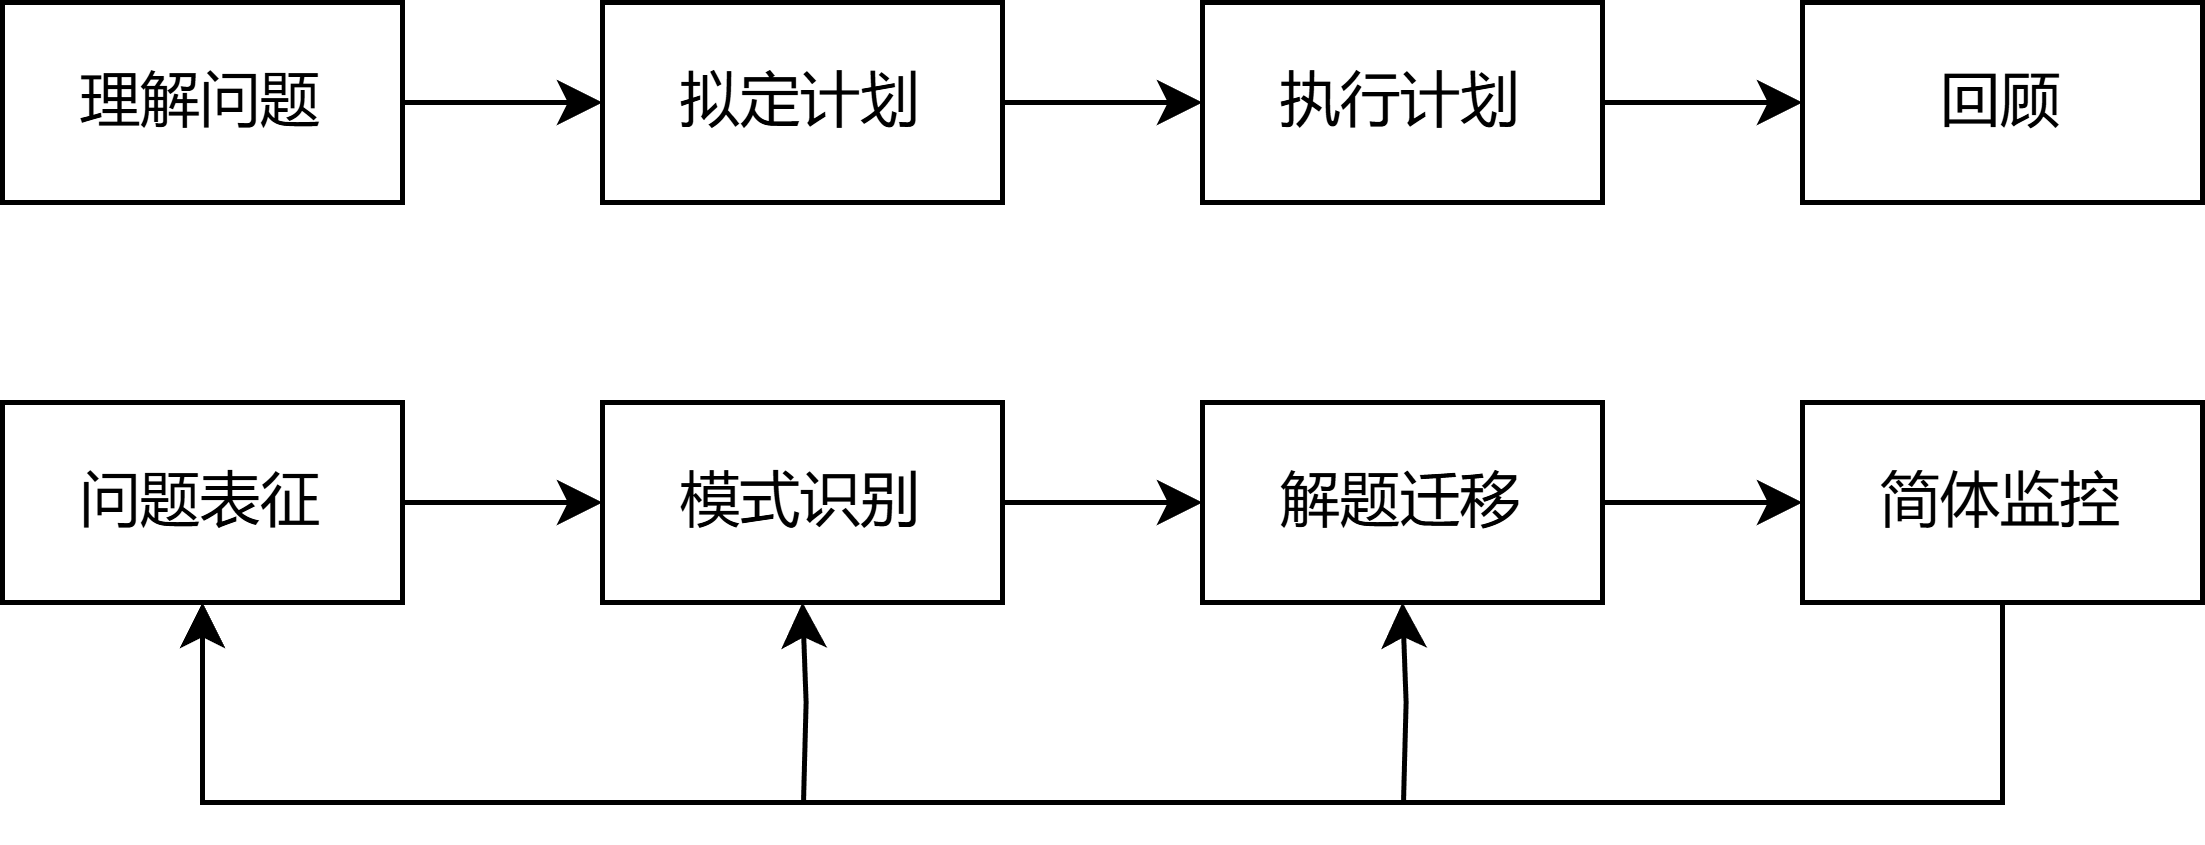
\includegraphics[width=0.5\linewidth]{image/数学解题教学模式.png}
    \caption{数学解题教学模式}
\end{figure}

\begin{itemize}
    \item 解题认知模式是一个系统。
    \item 解题认知系统是一个循环系统。
    \item 解题认知系统是一个控制系统。
\end{itemize}


\subsection{认知构建模式}

\begin{figure}[H]
    \centering
    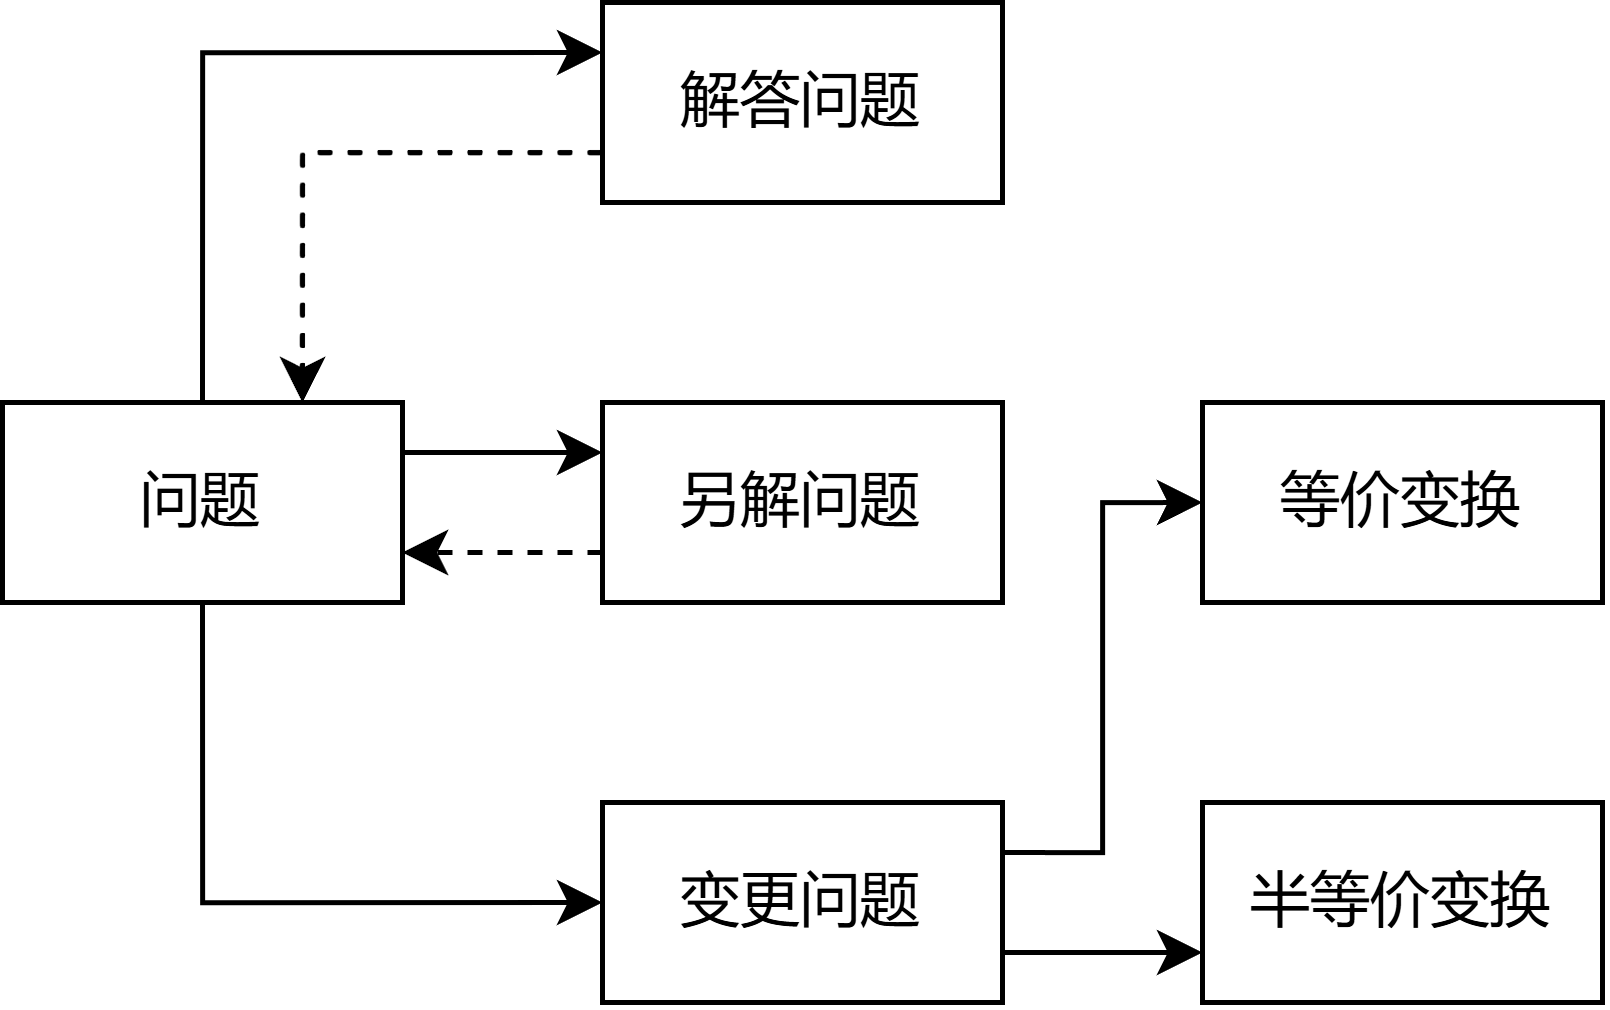
\includegraphics[width=0.35\linewidth]{image/认知构建模式.png}
\end{figure}

\begin{itemize}
    \item 等价变化(对条件、结论、问题、图形等价变化)
    \item 半等价变化(加强/减弱原问题的条件)
\end{itemize}

\textbf{注意事项}
\begin{enumerate}
    \item 问题要典型,可多法解决。
    \item 教师的作用在于诱导,体现学生主体性。
    \item 教学形式、手段多样化。
\end{enumerate}




\subsection{自动化技能形成模式}

\begin{figure}[H]
    \centering
    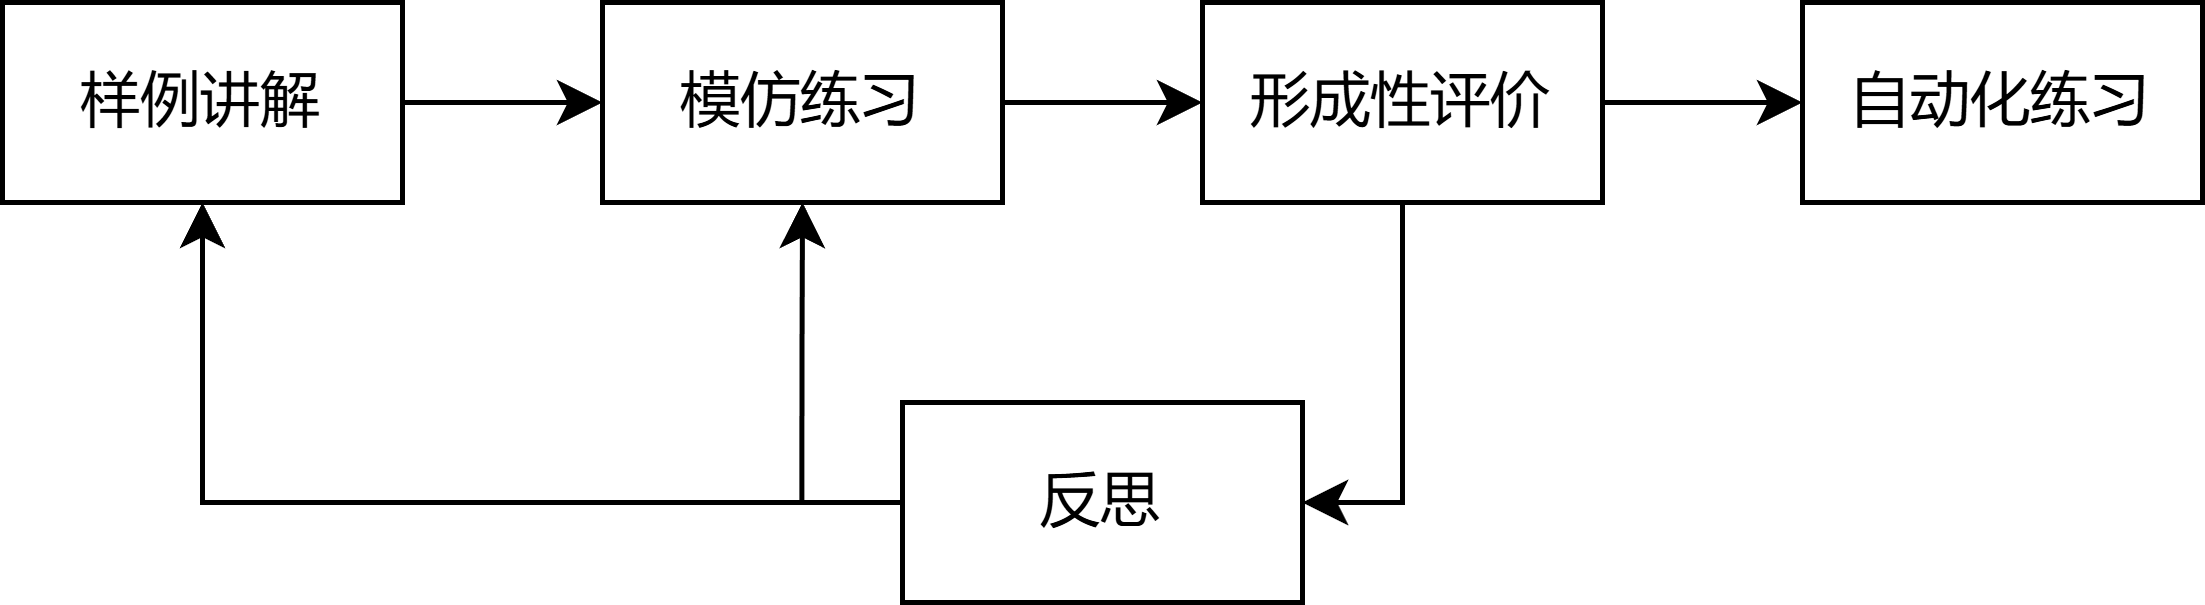
\includegraphics[width=0.5\linewidth]{image/自动化技能形成模式.png}
\end{figure}

\subsection{模型构建模式}

\begin{figure}[H]
    \centering
    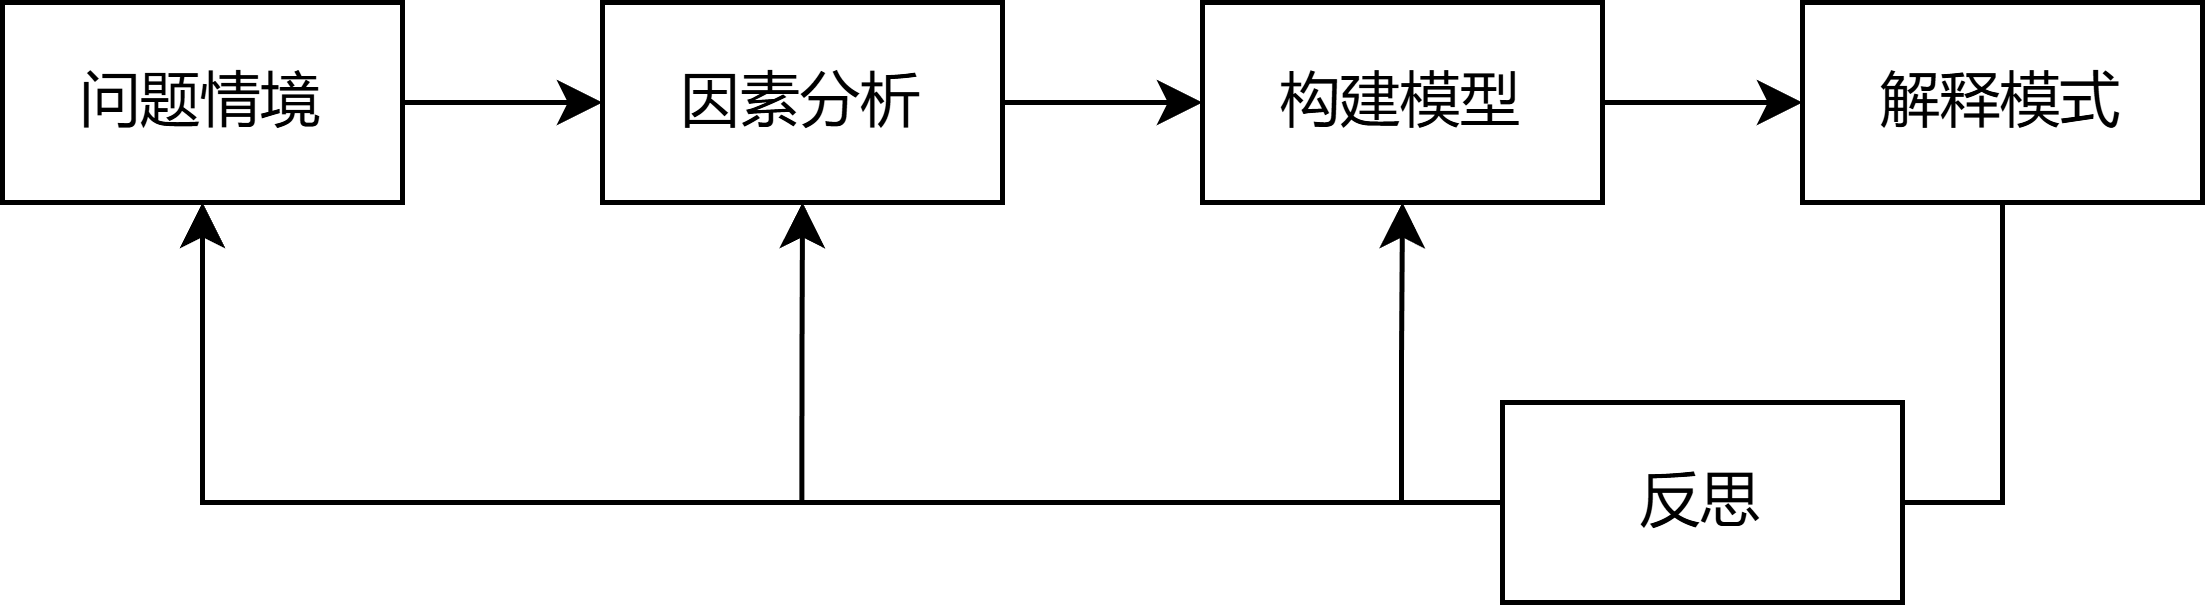
\includegraphics[width=0.5\linewidth]{image/模型构建模式.png}
\end{figure}

\subsection{问题开放模式}

\begin{figure}[H]
    \centering
    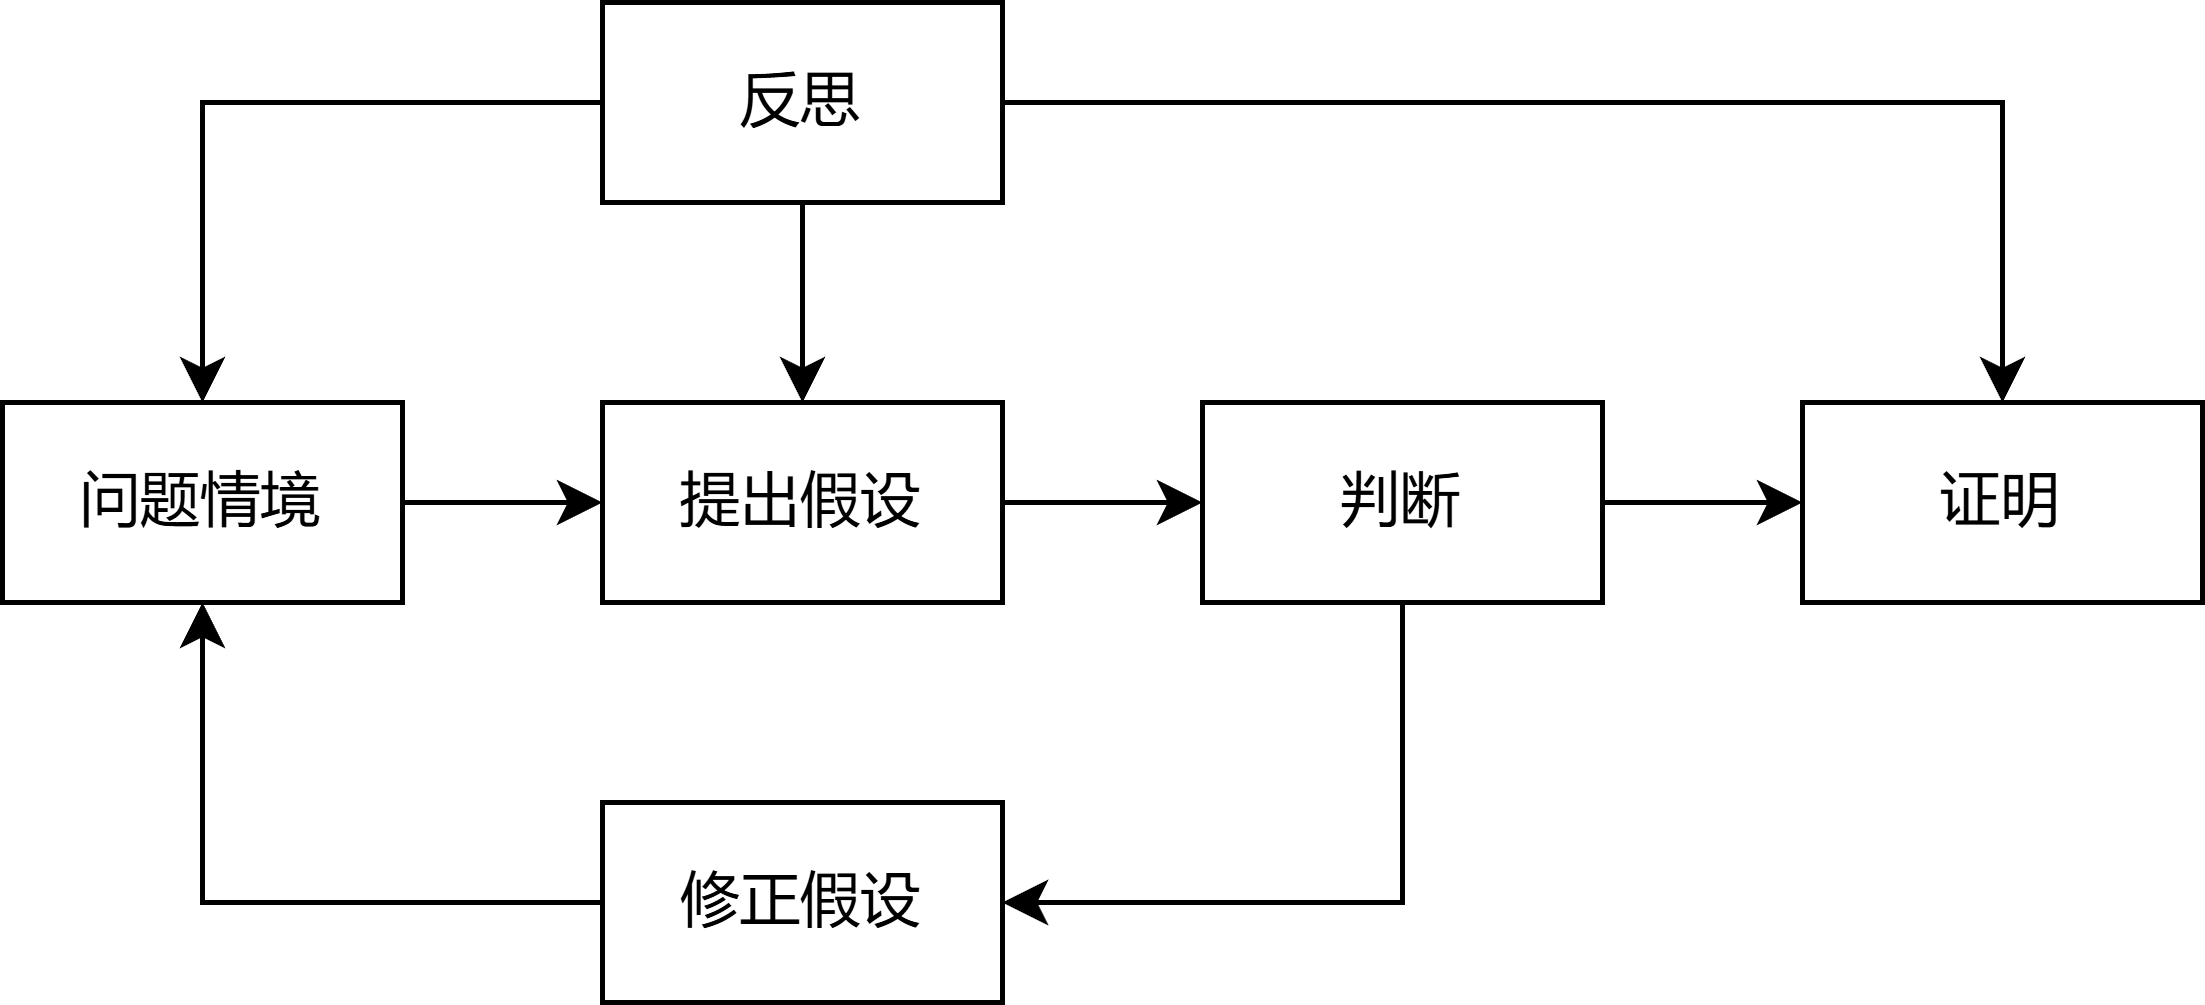
\includegraphics[width=0.5\linewidth]{image/问题开放模式.png}
\end{figure}